% Options for packages loaded elsewhere
\PassOptionsToPackage{unicode}{hyperref}
\PassOptionsToPackage{hyphens}{url}
%
\documentclass[
]{article}
\usepackage{lmodern}
\usepackage{amssymb,amsmath}
\usepackage{ifxetex,ifluatex}
\ifnum 0\ifxetex 1\fi\ifluatex 1\fi=0 % if pdftex
  \usepackage[T1]{fontenc}
  \usepackage[utf8]{inputenc}
  \usepackage{textcomp} % provide euro and other symbols
\else % if luatex or xetex
  \usepackage{unicode-math}
  \defaultfontfeatures{Scale=MatchLowercase}
  \defaultfontfeatures[\rmfamily]{Ligatures=TeX,Scale=1}
\fi
% Use upquote if available, for straight quotes in verbatim environments
\IfFileExists{upquote.sty}{\usepackage{upquote}}{}
\IfFileExists{microtype.sty}{% use microtype if available
  \usepackage[]{microtype}
  \UseMicrotypeSet[protrusion]{basicmath} % disable protrusion for tt fonts
}{}
\makeatletter
\@ifundefined{KOMAClassName}{% if non-KOMA class
  \IfFileExists{parskip.sty}{%
    \usepackage{parskip}
  }{% else
    \setlength{\parindent}{0pt}
    \setlength{\parskip}{6pt plus 2pt minus 1pt}}
}{% if KOMA class
  \KOMAoptions{parskip=half}}
\makeatother
\usepackage{xcolor}
\IfFileExists{xurl.sty}{\usepackage{xurl}}{} % add URL line breaks if available
\IfFileExists{bookmark.sty}{\usepackage{bookmark}}{\usepackage{hyperref}}
\hypersetup{
  pdftitle={Building Ensemble Models},
  pdfauthor={Xiaoyong Pan, Jenna Reps, Peter R. Rijnbeek},
  hidelinks,
  pdfcreator={LaTeX via pandoc}}
\urlstyle{same} % disable monospaced font for URLs
\usepackage[margin=1in]{geometry}
\usepackage{color}
\usepackage{fancyvrb}
\newcommand{\VerbBar}{|}
\newcommand{\VERB}{\Verb[commandchars=\\\{\}]}
\DefineVerbatimEnvironment{Highlighting}{Verbatim}{commandchars=\\\{\}}
% Add ',fontsize=\small' for more characters per line
\usepackage{framed}
\definecolor{shadecolor}{RGB}{248,248,248}
\newenvironment{Shaded}{\begin{snugshade}}{\end{snugshade}}
\newcommand{\AlertTok}[1]{\textcolor[rgb]{0.94,0.16,0.16}{#1}}
\newcommand{\AnnotationTok}[1]{\textcolor[rgb]{0.56,0.35,0.01}{\textbf{\textit{#1}}}}
\newcommand{\AttributeTok}[1]{\textcolor[rgb]{0.77,0.63,0.00}{#1}}
\newcommand{\BaseNTok}[1]{\textcolor[rgb]{0.00,0.00,0.81}{#1}}
\newcommand{\BuiltInTok}[1]{#1}
\newcommand{\CharTok}[1]{\textcolor[rgb]{0.31,0.60,0.02}{#1}}
\newcommand{\CommentTok}[1]{\textcolor[rgb]{0.56,0.35,0.01}{\textit{#1}}}
\newcommand{\CommentVarTok}[1]{\textcolor[rgb]{0.56,0.35,0.01}{\textbf{\textit{#1}}}}
\newcommand{\ConstantTok}[1]{\textcolor[rgb]{0.00,0.00,0.00}{#1}}
\newcommand{\ControlFlowTok}[1]{\textcolor[rgb]{0.13,0.29,0.53}{\textbf{#1}}}
\newcommand{\DataTypeTok}[1]{\textcolor[rgb]{0.13,0.29,0.53}{#1}}
\newcommand{\DecValTok}[1]{\textcolor[rgb]{0.00,0.00,0.81}{#1}}
\newcommand{\DocumentationTok}[1]{\textcolor[rgb]{0.56,0.35,0.01}{\textbf{\textit{#1}}}}
\newcommand{\ErrorTok}[1]{\textcolor[rgb]{0.64,0.00,0.00}{\textbf{#1}}}
\newcommand{\ExtensionTok}[1]{#1}
\newcommand{\FloatTok}[1]{\textcolor[rgb]{0.00,0.00,0.81}{#1}}
\newcommand{\FunctionTok}[1]{\textcolor[rgb]{0.00,0.00,0.00}{#1}}
\newcommand{\ImportTok}[1]{#1}
\newcommand{\InformationTok}[1]{\textcolor[rgb]{0.56,0.35,0.01}{\textbf{\textit{#1}}}}
\newcommand{\KeywordTok}[1]{\textcolor[rgb]{0.13,0.29,0.53}{\textbf{#1}}}
\newcommand{\NormalTok}[1]{#1}
\newcommand{\OperatorTok}[1]{\textcolor[rgb]{0.81,0.36,0.00}{\textbf{#1}}}
\newcommand{\OtherTok}[1]{\textcolor[rgb]{0.56,0.35,0.01}{#1}}
\newcommand{\PreprocessorTok}[1]{\textcolor[rgb]{0.56,0.35,0.01}{\textit{#1}}}
\newcommand{\RegionMarkerTok}[1]{#1}
\newcommand{\SpecialCharTok}[1]{\textcolor[rgb]{0.00,0.00,0.00}{#1}}
\newcommand{\SpecialStringTok}[1]{\textcolor[rgb]{0.31,0.60,0.02}{#1}}
\newcommand{\StringTok}[1]{\textcolor[rgb]{0.31,0.60,0.02}{#1}}
\newcommand{\VariableTok}[1]{\textcolor[rgb]{0.00,0.00,0.00}{#1}}
\newcommand{\VerbatimStringTok}[1]{\textcolor[rgb]{0.31,0.60,0.02}{#1}}
\newcommand{\WarningTok}[1]{\textcolor[rgb]{0.56,0.35,0.01}{\textbf{\textit{#1}}}}
\usepackage{graphicx,grffile}
\makeatletter
\def\maxwidth{\ifdim\Gin@nat@width>\linewidth\linewidth\else\Gin@nat@width\fi}
\def\maxheight{\ifdim\Gin@nat@height>\textheight\textheight\else\Gin@nat@height\fi}
\makeatother
% Scale images if necessary, so that they will not overflow the page
% margins by default, and it is still possible to overwrite the defaults
% using explicit options in \includegraphics[width, height, ...]{}
\setkeys{Gin}{width=\maxwidth,height=\maxheight,keepaspectratio}
% Set default figure placement to htbp
\makeatletter
\def\fps@figure{htbp}
\makeatother
\setlength{\emergencystretch}{3em} % prevent overfull lines
\providecommand{\tightlist}{%
  \setlength{\itemsep}{0pt}\setlength{\parskip}{0pt}}
\setcounter{secnumdepth}{5}
\usepackage{fancyhdr}
\pagestyle{fancy}
\fancyhead{}
\fancyhead[CO,CE]{Installation Guide}
\fancyfoot[CO,CE]{PatientLevelPrediction Package Version 3.1.0}
\fancyfoot[LE,RO]{\thepage}
\renewcommand{\headrulewidth}{0.4pt}
\renewcommand{\footrulewidth}{0.4pt}

\title{Building Ensemble Models}
\author{Xiaoyong Pan, Jenna Reps, Peter R. Rijnbeek}
\date{2020-06-03}

\begin{document}
\maketitle

{
\setcounter{tocdepth}{2}
\tableofcontents
}
\hypertarget{introduction}{%
\section{Introduction}\label{introduction}}

Ensemble models combine several models to improve the overall
performance. Traditionally, weak learners were combined to boost
performance but recent results show that combining several strong
approaches can also result in a better performance. There are many
examples in literature where ensemble models outperform individual
models using stacking, i.e.~a final logistic regresssion layer accross
the individual model outputs, but other approaches like weigthing has
also shown promising results.

This vignette describes how you can use the Observational Health Data
Sciencs and Informatics (OHDSI)
\href{http://github.com/OHDSI/PatientLevelPrediction}{\texttt{PatientLevelPrediction}}
package to build ensemble models. This vignette assumes you have read
and are comfortable with building single patient level prediction models
as described in the
\href{https://github.com/OHDSI/PatientLevelPrediction/blob/master/inst/doc/BuildingPredictiveModels.pdf}{\texttt{BuildingPredictiveModels}
vignette}.

This will enable studying ensemble methods at scale in the OHDSI data
network.

\begin{figure}
\centering
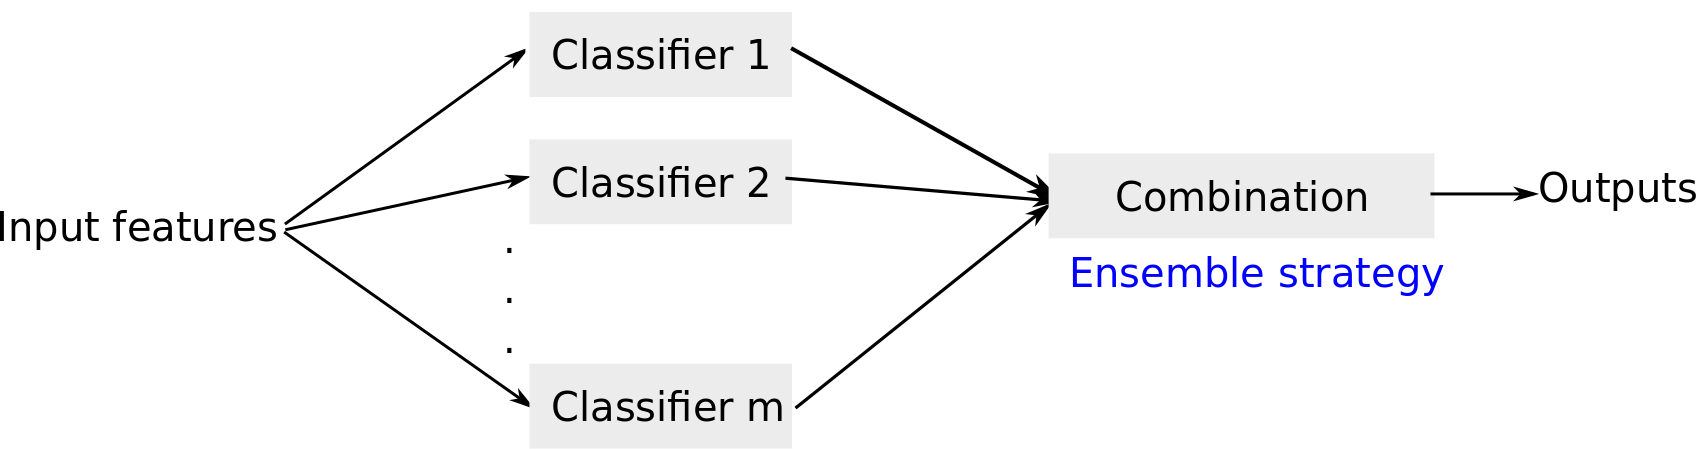
\includegraphics{ensemble.png}
\caption{Ensemble model}
\end{figure}

In PatientLevelPrediction package, four ensemble strategies have been
implemented:

\begin{enumerate}
\def\labelenumi{\arabic{enumi}.}
\tightlist
\item
  average ensemble: Calculate the average probability from individual
  models
\item
  product ensemble: Calculate the product of probabilites from
  individual models.
\item
  weighted ensemble: Calculate the weighted average probability from
  individual models using train AUC as weights.
\item
  stacked ensemble: Train a logistics regression on outputs from
  individual models
\end{enumerate}

\hypertarget{usage}{%
\section{Usage}\label{usage}}

Use the
\href{http://github.com/OHDSI/PatientLevelPrediction}{\texttt{PatientLevelPrediction}}
package to generate a \texttt{population} and \texttt{plpData} object.
Alternatively, you can make use of the data simulator. The following
code snippet creates a population of 12000 patients.

\begin{Shaded}
\begin{Highlighting}[]
\KeywordTok{data}\NormalTok{(plpDataSimulationProfile)}
\KeywordTok{set.seed}\NormalTok{(}\DecValTok{1234}\NormalTok{)}
\NormalTok{sampleSize <-}\StringTok{ }\DecValTok{2000}
\NormalTok{plpData <-}\StringTok{ }\KeywordTok{simulatePlpData}\NormalTok{(}
\NormalTok{  plpDataSimulationProfile,}
  \DataTypeTok{n =}\NormalTok{ sampleSize}
\NormalTok{)}

\NormalTok{population <-}\StringTok{ }\KeywordTok{createStudyPopulation}\NormalTok{(}
\NormalTok{  plpData,}
  \DataTypeTok{outcomeId =} \DecValTok{2}\NormalTok{,}
  \DataTypeTok{binary =} \OtherTok{TRUE}\NormalTok{,}
  \DataTypeTok{firstExposureOnly =} \OtherTok{FALSE}\NormalTok{,}
  \DataTypeTok{washoutPeriod =} \DecValTok{0}\NormalTok{,}
  \DataTypeTok{removeSubjectsWithPriorOutcome =} \OtherTok{FALSE}\NormalTok{,}
  \DataTypeTok{priorOutcomeLookback =} \DecValTok{99999}\NormalTok{,}
  \DataTypeTok{requireTimeAtRisk =} \OtherTok{FALSE}\NormalTok{,}
  \DataTypeTok{minTimeAtRisk =} \DecValTok{0}\NormalTok{,}
  \DataTypeTok{riskWindowStart =} \DecValTok{0}\NormalTok{,}
  \DataTypeTok{addExposureDaysToStart =} \OtherTok{FALSE}\NormalTok{,}
  \DataTypeTok{riskWindowEnd =} \DecValTok{365}\NormalTok{,}
  \DataTypeTok{addExposureDaysToEnd =} \OtherTok{FALSE}\NormalTok{,}
  \DataTypeTok{verbosity =} \StringTok{"INFO"}
\NormalTok{)}
\end{Highlighting}
\end{Shaded}

Specify the prediction algorithms to be combined.

\begin{Shaded}
\begin{Highlighting}[]
\CommentTok{# Use LASSO logistic regression and Random Forest as base predictors}
\NormalTok{model1 <-}\StringTok{ }\KeywordTok{setLassoLogisticRegression}\NormalTok{()}
\NormalTok{model2 <-}\StringTok{ }\KeywordTok{setRandomForest}\NormalTok{()}
\end{Highlighting}
\end{Shaded}

Specify a test fraction and a sequence of training set fractions.

\begin{Shaded}
\begin{Highlighting}[]
\NormalTok{testFraction <-}\StringTok{ }\FloatTok{0.2}
\end{Highlighting}
\end{Shaded}

Specify an ensembleStrategy to combine multiple predictors. The strategy
used for ensembling the outputs from different models, it can be `mean',
`product', `weighted' and `stacked': `mean' the average probability from
differnt models `product' the product rule `weighted' the weighted
average probability from different models using train AUC as weights.
`stacked' the stakced ensemble trains a logistics regression on
different models.

\begin{Shaded}
\begin{Highlighting}[]
\NormalTok{ensembleStrategy <-}\StringTok{ 'stacked'}
\end{Highlighting}
\end{Shaded}

Specify the test split to be used.

\begin{Shaded}
\begin{Highlighting}[]
\CommentTok{# Use a split by person, alterantively a time split is possible}
\NormalTok{testSplit <-}\StringTok{ 'person'}
\end{Highlighting}
\end{Shaded}

Run the ensemble learning to combine model1 and model2. You can also use
different plpData for different models.

\begin{Shaded}
\begin{Highlighting}[]
\NormalTok{ensembleResults <-}\StringTok{ }\NormalTok{PatientLevelPrediction}\OperatorTok{::}\KeywordTok{runEnsembleModel}\NormalTok{(population, }
                                   \DataTypeTok{dataList =} \KeywordTok{list}\NormalTok{(plpData, plpData), }
                                   \DataTypeTok{modelList =} \KeywordTok{list}\NormalTok{(model1, model2),}
                                   \DataTypeTok{testSplit=}\NormalTok{testSplit,}
                                   \DataTypeTok{testFraction=}\NormalTok{testFraction,}
                                   \DataTypeTok{nfold=}\DecValTok{3}\NormalTok{, }\DataTypeTok{splitSeed=}\DecValTok{1000}\NormalTok{, }
                                   \DataTypeTok{ensembleStrategy =}\NormalTok{ ensembleStrategy) }
\end{Highlighting}
\end{Shaded}

\hypertarget{saving-and-loading-the-ensemble-model}{%
\subsection{Saving and loading the ensemble
model}\label{saving-and-loading-the-ensemble-model}}

You can save and load the model using:

\begin{Shaded}
\begin{Highlighting}[]
\KeywordTok{saveEnsemblePlpModel}\NormalTok{(ensembleResults}\OperatorTok{$}\NormalTok{model, }\DataTypeTok{dirPath =} \KeywordTok{file.path}\NormalTok{(}\KeywordTok{getwd}\NormalTok{(), }\StringTok{"model"}\NormalTok{))}
\NormalTok{ensembleModel <-}\StringTok{ }\KeywordTok{loadEnsemblePlpModel}\NormalTok{(}\KeywordTok{getwd}\NormalTok{(), }\StringTok{"model"}\NormalTok{)}
\end{Highlighting}
\end{Shaded}

\hypertarget{apply-ensemble-model}{%
\section{Apply Ensemble model}\label{apply-ensemble-model}}

\begin{Shaded}
\begin{Highlighting}[]
\NormalTok{plpData <-}\StringTok{ }\KeywordTok{loadPlpData}\NormalTok{(}\StringTok{"<data file>"}\NormalTok{)}
\NormalTok{populationSettings <-}\StringTok{ }\NormalTok{ensembleModel}\OperatorTok{$}\NormalTok{populationSettings}
\NormalTok{populationSettings}\OperatorTok{$}\NormalTok{plpData <-}\StringTok{ }\NormalTok{plpData}
\NormalTok{population <-}\StringTok{ }\KeywordTok{do.call}\NormalTok{(createStudyPopulation, populationSettings)}
\end{Highlighting}
\end{Shaded}

Load the model.

\begin{Shaded}
\begin{Highlighting}[]
\NormalTok{ensembleModel <-}\StringTok{ }\KeywordTok{loadEnsemblePlpModel}\NormalTok{(}\StringTok{"<model folder>"}\NormalTok{)}
\end{Highlighting}
\end{Shaded}

Get the predictions by applying the model:

\begin{Shaded}
\begin{Highlighting}[]
\NormalTok{prediction <-}\StringTok{ }\KeywordTok{applyEnsembleModel}\NormalTok{(population,}
                                  \DataTypeTok{dataList =} \KeywordTok{list}\NormalTok{(plpData, plpData),}
                                  \DataTypeTok{ensembleModel =}\NormalTok{ ensembleModel)}\OperatorTok{$}\NormalTok{prediction}
\end{Highlighting}
\end{Shaded}

\hypertarget{demo}{%
\section{Demo}\label{demo}}

We have added a demo of the ensemble training:

\begin{Shaded}
\begin{Highlighting}[]
\CommentTok{# Show all demos in our package: }
 \KeywordTok{demo}\NormalTok{(}\DataTypeTok{package =} \StringTok{"PatientLevelPrediction"}\NormalTok{)}

\CommentTok{# Run the learning curve}
 \KeywordTok{demo}\NormalTok{(}\StringTok{"EnsembleModelDemo"}\NormalTok{, }\DataTypeTok{package =} \StringTok{"PatientLevelPrediction"}\NormalTok{)}
\end{Highlighting}
\end{Shaded}

\hypertarget{acknowledgments}{%
\section{Acknowledgments}\label{acknowledgments}}

Considerable work has been dedicated to provide the
\texttt{PatientLevelPrediction} package.

\begin{Shaded}
\begin{Highlighting}[]
\KeywordTok{citation}\NormalTok{(}\StringTok{"PatientLevelPrediction"}\NormalTok{)}
\end{Highlighting}
\end{Shaded}

\begin{verbatim}
## 
## To cite PatientLevelPrediction in publications use:
## 
## Reps JM, Schuemie MJ, Suchard MA, Ryan PB, Rijnbeek P (2018). "Design and
## implementation of a standardized framework to generate and evaluate patient-level
## prediction models using observational healthcare data." _Journal of the American
## Medical Informatics Association_, *25*(8), 969-975. <URL:
## https://doi.org/10.1093/jamia/ocy032>.
## 
## A BibTeX entry for LaTeX users is
## 
##   @Article{,
##     author = {J. M. Reps and M. J. Schuemie and M. A. Suchard and P. B. Ryan and P. Rijnbeek},
##     title = {Design and implementation of a standardized framework to generate and evaluate patient-level prediction models using observational healthcare data},
##     journal = {Journal of the American Medical Informatics Association},
##     volume = {25},
##     number = {8},
##     pages = {969-975},
##     year = {2018},
##     url = {https://doi.org/10.1093/jamia/ocy032},
##   }
\end{verbatim}

\textbf{Please reference this paper if you use the PLP Package in your
work:}

\href{http://dx.doi.org/10.1093/jamia/ocy032}{Reps JM, Schuemie MJ,
Suchard MA, Ryan PB, Rijnbeek PR. Design and implementation of a
standardized framework to generate and evaluate patient-level prediction
models using observational healthcare data. J Am Med Inform Assoc.
2018;25(8):969-975.}

\end{document}
